\title{Computer Networks - CS 204} % You may change the title if you want.

\author{Rishit Saiya - 180010027, Summary}

\date{\today}

\documentclass[12pt]{article}
\usepackage{fullpage}
\usepackage{enumitem}
\usepackage{amsmath,mathtools}
\usepackage{amssymb}
\usepackage[super]{nth}
\usepackage{textcomp}
\usepackage{hyperref}
\usepackage{soul}
\begin{document}
\maketitle

%-------------------------------------------------------------------------
\section{Random Access MAC Protocols}
These protocols are taken into considerations when transmission is at full channel data rate. Moreover, there is no coordination between prior nodes and current nodes. From previous literature, it is clear that 2 or more nodes transmitting at the same time will lead to collision in the network.

These protocols specify and lead us to detect collisions and how to mitigate and recover from the collisions. Examples of Random Access Protocols are ALOHA, Slotted ALOHA, CSMA $\And$ CSMA/CD.

%-------------------------------------------------------------------------

\section{ALOHA}
The crude idea of the ALOHA protocol was as follows: \\

Whenever the sender is ready, it transmits the packet. Receiver then sends a ACK back to the sender. There is timings maintained for each ACK. This idea is in resemblance with the Congestion Control detection with timings attached to ACKs. Next here, collision are detected with timings of the ACKs. Recovery from the collision is by trying after random delay (Backoff Approach).

% \textbf{\textit{If the delay is too short/too longs :- cases to be written. Doubt.}} 

When the implementation of ALOHA was shifted from pure to slotted, we had rise in utilization with $36\%$ from $18\%$.

It is depicted in Figure 1.

\begin{figure}
    \centering
    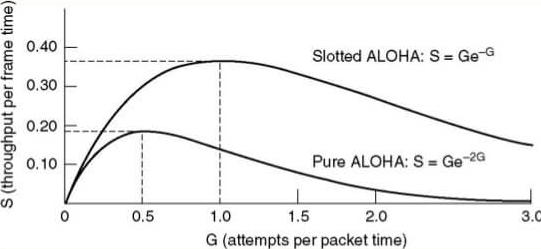
\includegraphics[width=10cm, height=5cm]{aloha.png}
    \caption{Throughput Vs. Offered Traffic for Pure ALOHA and Slotted ALOHA}
\end{figure}

\subsection{Slotted ALOHA}
The working of Slotted ALOHA is as follows: 
\begin{itemize}
    \item The packet transmission time is divided into equal size slots.
    \item A node transmits the packet at the beginning of the next slot.
    \item If a collision occurs, the node retransmits the packet in future slots with probability ‘p’ until we have a successful transmission.
\end{itemize}

\subsection{Pure ALOHA}
This is basically unslotted, just the quite opposite of Slotted ALOHA. The working in Pure ALOHA is as follows:
\begin{itemize}
    \item The packet is transmitted without awaiting for beginning of the slot.
    \item It is natural that in these cases, the chances of collisions increase tremendously. A simple collision example can be explained as follows: \\ 
    Consider a packet sent at a certain time $t_0$ will collide with the packets sent at the times [$t_0-1$ , $t_0+1$] because the packet at time $t_0$ will have an overlap with the packets of times [$t_0-1$ , $t_0+1$] in the time frames.
    
\end{itemize}

%-------------------------------------------------------------------------

\section{Ethernet}

This first practical LAN (Local Area Network) was the Ethernet.

The basic idea was remains the same. It had to listen to the wire before transmission. If a collision is detected, it is avoided in the active transmission time.

\subsection{Ethernet MAC Protocols}
In ALOHA, decisions to transmit are made irrespective of other nodes' involvement in the network. Ethernet uses CSMA/CD and listens to line before or during the process of transmission. \\

If the line is idle, the condition is said to be no carrier sensed. In this case, we send packet immediately. It is to be noted that the upper bound message size of \textbf{\textit{1500 bytes}} and the line in the network has to wait for \textbf{\textit{9.6 $\mu sec$}}.  \\

If the line is busy, the condition is said to be carrier sensed. We wait until the line is idle again and transmit the packet immediately afterwards. \\

If collision is detected, we stop sending packets due to the jam signal. We try again later.

\subsection{10Base2 Ethernet Technology}
The \textbf{10} represents the 10 Mbps and \textbf{2} represents the ($\sim$ 200 meters) cable length. The cable is coaxial in nature and is used in Bus Topology. Repeaters are used to connect to multiple segments. The physical layer device, Repeater repeats bits it receives on one interface onto the other interfaces.

\subsection{10BaseT Ethernet Technology}
The \textbf{10} represents the 10 Mbps and \textbf{T} stands for the Twisted Pair. The hubs are connected by Twisted Pair Facility in a Star Network Topology given that the distance between any node to hub is less than 100m.

\subsection{100BaseT Ethernet Technology}
The \textbf{100} represents the 100 Mbps and \textbf{T} stands for the Twisted Pair. The hubs are connected by Twisted Pair Facility in a Star Network Topology given that the distance between any node to hub is less than 100m.


\subsection{Ethernet Frame Format}
The Ethernet Frame Format is divided into 2 types based on the guidelines and compliance it was set in. They are explained as follows.
\begin{enumerate}
    \item \textbf{The Ethernet MAC Frame Format} \\
        The Ethernet MAC Frame Format is as given in Figure 2.
        \begin{figure}
            \centering
            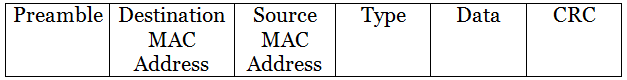
\includegraphics[width=15cm, height=2cm]{ethernet_frame.png}
            \caption{Ethernet MAC Frame Format}
        \end{figure}
        
        The components in the Ethernet Frame are explained as follows:
        \begin{itemize}
            \item \textbf{\textit{Preamble}} \\
                It is used to synchronize the receiver before actual data is sent. It consists of a sequence of 7 bytes, each set to 1010101.
            \item \textbf{\textit{MAC Addresses (Source and Destination)}} \\
                It is a unique, 48-bit unicast address assigned to each adapter. Example: D4-3B-04-67-16-AE.
            \item \textbf{\textit{Type}} \\
                This field is a demultiplexing key used to determine which higher level protocol the frame should be delivered to.
            \item \textbf{\textit{Body}} \\
                The body is the field which has the capacity to contain upto 1500 bytes of data.
        \end{itemize}
        
    \item \textbf{The Ethernet IEEE 802.3 Frame Format} \\
    The Ethernet IEEE 802.3 Frame Format is as given in Figure 3.
        \begin{figure}
            \centering
            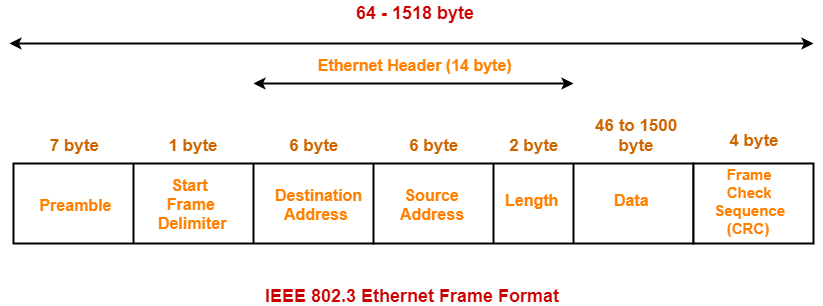
\includegraphics[width=15cm, height=5cm]{ethernet_frame_802.3.png}
            \caption{Ethernet IEEE 802.3 Frame Format}
        \end{figure}
        
        The components in the Ethernet Frame are explained as follows:
        \begin{itemize}
            \item \textbf{\textit{Preamble}} \\
                It informs the receiving system that a frame is starting and enables synchronization.
            \item \textbf{\textit{SFD (Start Frame Delimiter)}} \\
                It signifies that the destination MAC Address field begins with the next byte. This is a 1-Byte field which is always set to 10101011.
            \item \textbf{\textit{Destination MAC Address}} \\
                It identifies the receiving system.
            \item \textbf{\textit{Source MAC Address}} \\
                It identifies the sending system.
            \item \textbf{\textit{Type}} \\
                This field defines the type of protocol such as IPv4 or IPv6 inside the frame.
            \item \textbf{\textit{Data}} \\
                It contains the payload data. Padding Data is added to meet the minimum length requirement for this field (46 bytes).
            \item \textbf{\textit{FCS (Frame Check Sequence)}} \\
                It contains a 32-bit \textbf{\textit{Cyclic Redundancy Check (CRC)}} which allows detection of malicious data.
        \end{itemize}

\end{enumerate}

%----------------------------------------------------------------------------

\section{Collision Detection}

% \subsection{Collision}
    A \textbf{Collision} is caused when two adapters transmit at the same time. The adapters in the network sense collision based on the voltage differences.

So far, all the things have been explained on how the protocols work when a collision is detected. But we also need to firmly understand how the collision is actually detected.

Consider two hosts, \textbf{A} $\And$ \textbf{B}, who belong to a certain network. Suppose A sends a packet which takes T time to reach B. WLOG, we can say that B's packet will also take T time to reach A. So if A is still transmitting at 2T, a collision is detected. This mechanism is in general used to detect collisions.

Using IEEE 802.3 standards, we specify maximum value of 2T to \textbf{\textit{51.2 $\mu sec$}}

%----------------------------------------------------------------------

\section{Exponential Backoff}
From previous literature, we are aware that if a collision is detected, we make a delay in the next sending packet and try again till it is successfully transmitted.

The delay time is decided using \textit{Binary Exponential Backoff}.
Based upon the number of delays, the delay time is selected as follows:
\begin{itemize}
    \item If checking $1^{st}$ time for transmission is leading to collision, then     the delay time is calculated by, K $\times$ 51.2 $\mu sec$, where K is         chosen from \{0,1\}.
    \item If checking $2^{nd}$ time for transmission is leading to collision, then     the delay time is calculated by, K $\times$ 51.2 $\mu sec$, where K is         chosen from \{0,1,2,3\}.
    \item If checking $n^{th}$ time for transmission is leading to collision, then     the delay time is calculated by, K $\times$ 51.2 $\mu sec$, where K is         chosen from \{0,1,2,3,...$2^n-1$\}. Note: $K_{max} = 1023$.
    \item After several tries, host reports a transmit error.
\end{itemize}
Given all this, if the delay is not random, then there is a chance that sources would retransmit in the lock step. WLOG, we can say that this works for small number of hosts. It is natural that large number of hosts manifest to large number of collisions.

%------------------------------------------------------------------------

\section{Ethernet Issues}
We need to understand the issues regarding the Ethernet so as to mitigate the collisions and try to upgrade the number of transmissions in a given time frame. The general issues are as follows:
\begin{itemize}
    \item Ethernet's peak utilization is pretty low. This is due to the     bandwidth used in the recoveries from the collisions, etc.
    \item The peak throughput/utilisation is worst with more number of hosts. It is natural that more number of hosts lead to more number of collisions.
    \item The peak throughput is worst with small packets size. This is because the recoveries for collisions would have to be frequent and that would lead to a huge loss in the bandwidth.
    \item Longer Links can result one more drawback in the peak throughput of Ethernet because the collision detection will take a lot time to reach to the hosts in the network resulting in late recoveries and wastage of bandwidth.
\end{itemize}

%------------------------------------------------------------------------

\section{Evolution of Ethernet}

With the motive of resolving above issues and advancing towards better Ethernet technologies, we have evolved towards various types of Ethernet based on bandwidth.

A picture depicting the evolution is in the Figure 4.
\begin{figure}
    \centering
    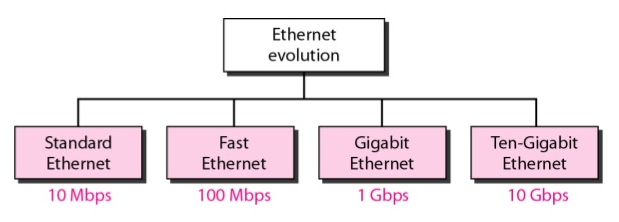
\includegraphics[width=15cm, height=5cm]{ethernet_evolution.png}
    \caption{Ethernet Evolution}
\end{figure}

The different types of modified Ethernet are:
\begin{itemize}
    \item \textbf{Bridged Ethernet} \\
        \begin{figure}
            \centering
            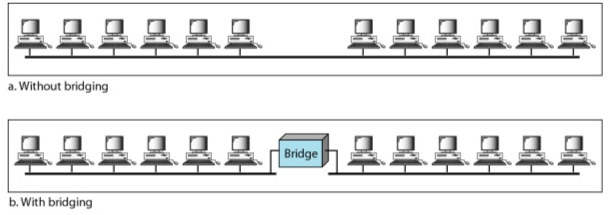
\includegraphics[width=15cm, height=5cm]{bridged_ethernet.png}
            \caption{Bridged vs. Non Bridged Ethernet}
        \end{figure}
        In bridged LANs, LAN is divided using bridges. This resulted in increased bandwidth and seperated the collision domains. As we can see in the Figure 5, if a collision occurs in a LAN in which bridge isn't present, it jams the whole LAN. On the other hand, if the collision occurs in the LAN with a bridge in it, it only happens only in a particular segment of the LAN and essentially jams only those stations where the collision has occurred, keeping other stations active for transmission.
    \item \textbf{Switched Ethernet} \\
        \begin{figure}
            \centering
            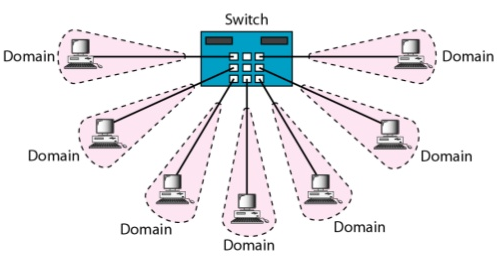
\includegraphics[width=10cm, height=5cm]{switched_ethernet.png}
            \caption{Switched Ethernet}
        \end{figure}
        This is basically extension of Bridged Ethernet. It is 2-way communication provider. Here a switch is provided to each domain in the LAN, so this acts as a mitigation to the incoming collisions as well as reduces the loss in the bandwidth.
    \item \textbf{Full-Duplex Switched Ethernet} \\
        \begin{figure}
            \centering
            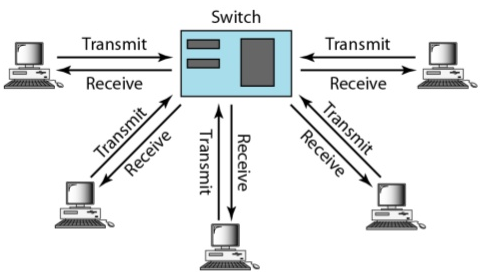
\includegraphics[width=10cm, height=5cm]{full_duplex_switched_ethernet.png}
            \caption{Full-Duplex Switched Ethernet}
        \end{figure}
        The 2 way communication with the switches and bridges gives a full-duplex switch ethernet. The 10BaseT Ethernet is a full-duplex switch ethernet whilst the 10Base5 and 10Base2 is half-duplex switch ethernet. The advantages of Full-Duplex Ethernet are as follows:
        \begin{itemize}
            \item Eradicating CSMA/CD \\
                In Full-Duplex Switch Ethernet, each station is connected to the switch via 2 separate links. Each link is point-to-point dedicated path between the station and the switch. 
            \item Addition of MAC Control Layer \\
                To provide a flow and error control in full-duplex switched ethernet, a new sublayer, called MAC Control Layer is introduced between LLC $\And$ MAC sublayers. This is because Standard Ethernet was designed as a connectionless protocol at the MAC layer.
        \end{itemize}
    \item \textbf{Fast Ethernet} \\
        The fast Ethernet is just with the goal of increasing the internet speed providing upto 100 Mbps.
    \item \textbf{Gigabit Ethernet} \\
        The Gigabit Ethernet is just with the goal of increasing the internet speed providing upto 1000 Mbps.
\end{itemize}
%-------------------------------------------------------------------------

\section{Ethernet Addressing}

Each network device/station on an Ethernet network has its own Network Interface Card (NIC). All the devices connected to the network are manufactured in such a way that NIC is fitted inside the station and provides the station with a 6-byte physical address.

For example: D3-3B-10-06-16-AE

According to the scheme at Data Link Layer, the Ethernet Addresses have been divided as follows:
\begin{itemize}
    \item \textbf{\textit{Unicast Address}} \\
        A source address is always a unicast address because the frame comes only from 1 station. When destination address is considered, if the last bit (or Least Significant Bit) of $1^{st}$ byte of Ethernet Address in binary form is 0, then it is classified under Unicast Address.
    \item \textbf{\textit{Multicast Address}} \\    
        In the destination Address, if the last bit (or Least Significant Bit) of $1^{st}$ byte of Ethernet Address in binary form is \textbf{not} 0, then it is classified under Multicast Address.
    \item \textbf{\textit{Broadcast Address}} \\
        A special case of Multicast Address is Broadcast Address, where all the bits in the $1^{st}$ byte are 1s.
\end{itemize}
\textbf{Example:} D3-3B-10-06-16-AE \\
The binary form of above address is 1101001\textbf{\underline{1}}-00111011-00010000-00000110-00010110-10101110
The last bit of $1^{st}$ byte is underlined above. Since it is 1, it is classified under Multicast Address.

%-----------------------------------------------------------------------

\end{document}